%
% File eacl2017.tex
%
%% Based on the style files for ACL-2016
%% Based on the style files for ACL-2015, with some improvements
%%  taken from the NAACL-2016 style
%% Based on the style files for ACL-2014, which were, in turn,
%% Based on the style files for ACL-2013, which were, in turn,
%% Based on the style files for ACL-2012, which were, in turn,
%% based on the style files for ACL-2011, which were, in turn, 
%% based on the style files for ACL-2010, which were, in turn, 
%% based on the style files for ACL-IJCNLP-2009, which were, in turn,
%% based on the style files for EACL-2009 and IJCNLP-2008...

%% Based on the style files for EACL 2006 by 
%%e.agirre@ehu.es or Sergi.Balari@uab.es
%% and that of ACL 08 by Joakim Nivre and Noah Smith

\documentclass[11pt]{article}
\usepackage{eacl2017}
\usepackage{times}
\usepackage{url}
\usepackage{latexsym}
\usepackage{graphicx}
\usepackage{color}
\usepackage{booktabs}

\eaclfinalcopy % Uncomment this line for the final submission
%\def\eaclpaperid{***} %  Enter the acl Paper ID here

%\setlength\titlebox{5cm}
% You can expand the titlebox if you need extra space
% to show all the authors. Please do not make the titlebox
% smaller than 5cm (the original size); we will check this
% in the camera-ready version and ask you to change it back.

\newcommand\BibTeX{B{\sc ib}\TeX}

\title{OpenNMT: Open-Source Toolkit for Neural Machine Translation}

\author{Guillaume Klein$^\dagger$, Yoon Kim$^*$, Yuntian Deng$^*$, Jean Senellart$^\dagger$, Alexander M. Rush$^*$ \\ Harvard University$^*$, SYSTRAN $^\dagger$}

\date{}

\begin{document}
\maketitle
\begin{abstract}

  We describe an open-source toolkit for neural machine translation
  (NMT).  The toolkit prioritizes efficiency, modularity, and
  extensibility with the goal of supporting NMT research into model
  architectures, feature representations, and source modalities, while
  maintaining competitive performance and reasonable training
  requirements. The toolkit consists of modeling and translation support,
  as well as detailed pedagogical documentation about the underlying
  techniques.

\end{abstract}

\section{Introduction}


Neural machine translation (NMT) is a new methodology for machine
translation that has led to remarkable improvements, particularly in
terms of human evaluation, compared to rule-based
and statistical machine translation (SMT) systems
\cite{wu2016google,systran}. Originally developed using pure
sequence-to-sequence models \cite{sutskever14sequence,Cho2014} and
improved upon using attention-based variants \cite{Bahdanau2015,Luong2015}, NMT has now become a widely-applied technique for machine
translation, as well as an effective approach for other related NLP
tasks such as dialogue, parsing, and summarization.

As NMT approaches are standardized, it becomes more important for the
machine translation and NLP community to develop open
implementations for researchers to benchmark against, learn from, and
extend upon. Just as the SMT community benefited greatly from toolkits
like Moses \cite{koehn2007moses} for phrase-based MT and the CDec
toolkit \cite{dyer2010cdec} for syntax-based MT, NMT toolkits can
provide a foundation for the research community. A toolkit should aim
to provide a shared framework for developing and comparing
open-source systems, while at the same time being
efficient and accurate enough to be used in production contexts.


\begin{figure}
  \centering
  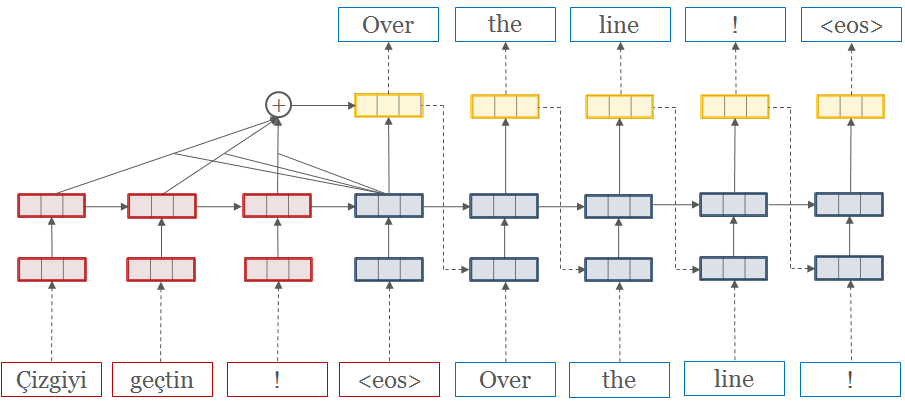
\includegraphics[width=\linewidth]{simple-attn}
  \label{fig:rnn}
  \caption{\small Schematic view of neural machine translation. The \textcolor{red}{red} source words are first mapped to word vectors and then fed into a recurrent neural network (RNN). Upon seeing the $\langle$eos$\rangle$ symbol, the final time step initializes a target \textcolor{blue}{blue} RNN. At each target time step, \textit{attention} is applied over the source RNN and combined with the current hidden state to produce a prediction $p(w_t| w_{1: t-1}, x)$ of the next word. This prediction is then fed back into the target RNN.}
\end{figure}

% In this work we describe a new open-source toolkit for developing
% neural machine translation systems, known as \textit{OpenNMT}. The
% system is motivated by frameworks, such as Moses and CDec developed
% for statistical machine translation (SMT). These toolkits aim to
% provide a shared frameworks for developing and comparing open-source
% SMT systems that are complete and flexible enough for research
% development, while at the same time being efficient and accurate
% enough to be used production contexts. 

Currently there are several existing NMT implementations. Many systems
such as those developed in industry by Google \cite{wu2016google},
Microsoft, and Baidu, are closed source, and are unlikely to be
released with unrestricted licenses. Many other systems such as
\textit{GroundHog}, \textit{Blocks}, \textit{tensorflow-seq2seq}, and our own \textit{seq2seq-attn}, exist
mostly as research code. These libraries provide important
functionality but minimal support to production users. Perhaps most
promising is the University of Edinburgh's \textit{Nematus} system originally based on NYU's NMT system. Nematus provides high-accuracy translation, many options,
clear documentation, and has been used in several successful research
projects. In the development of this project, we aimed to build upon the strengths of this system, while providing additional documentation and functionality to provide a
useful open-source NMT framework for the NLP community in academia and
industry.

With this goal in mind, we introduce \textit{OpenNMT} (\url{http://opennmt.net}), an open-source framework
for neural machine translation. OpenNMT is a complete NMT
implementation. In addition to providing code for the core translation
tasks, OpenNMT was designed with three aims:
(a) prioritize first training and test efficiency, (b) maintain model modularity and readability, (c) support significant research extensibility.

This report describes how the first-release of the
system targets these criteria. We begin by briefly surveying the
background for NMT, describing the high-level implementation details,
and then describing specific case studies for the three criteria.  We
end by showing preliminary benchmarks of the system in terms of
accuracy, speed, and memory usage for several translation and
translation-like tasks.

% the main aspects of system development, and the preliminary results from using the system in practice.  

% (a) Our top priority was training and decoding speed. NMT systems are
% notoriously slow to train, often requiring weeks of training time on
% the latest GPU hardware and significant test resources. We targeted
% this issue by implementing multi-GPU training, using aggressive memory
% sharing, and developing a specialized CPU decoder. 

% (b) Our second
% priority was system modularity and teachibility. We intend OpenNMT as
% a living research system, and so the codebase was developed to provide
% a self-documenting overview of NMT. We discuss how this approach
% allowed us to add factored models \cite{} to the system. 

% (c) Finally
% NMT is a very quick moving research area, and we would like the system
% to support new research areas as they develop. To demonstrate this
% approach we abstracted out the core of OpenNMT as a library, and
% describe the case study of using OpenNMT for image-to-text
% translation.




\section{Background}

NMT has now been extensively described in many
excellent tutorials (see for instance
\url{https://sites.google.com/site/acl16nmt/home}). We give
a condensed overview. 

NMT takes a conditional language modeling view of translation (as
opposed to the noisy channel view of SMT). Formally NMT models the
probability of a target sentence $w_{1:T}$ given a source sentence
$x_{1:S}$ as
$p(w_{1:T}| x) = \prod_{1}^T p(w_t| w_{1:t-1}, x; \theta)$. This
distribution is estimated using an attention-based encoder-decoder
architecture \cite{Bahdanau2015}. A source encoder recurrent neural
network (RNN) maps each source word to a word vector, and processes
these to a sequence of hidden vectors
$\mathbf{h}_1, \ldots, \mathbf{h}_S$.  The target decoder combines an
RNN hidden representation of previously generated words
($w_1, ... w_{t-1}$) with source hidden vectors to predict scores for
each possible next word. A softmax layer is then used to produce a
next-word distribution $ p(w_t| w_{1:t-1}, x; \theta)$. The source
hidden vectors influence the distribution through an attention pooling
layer that weights each source word relative to its expected
contribution to the target prediction. The complete model is trained
end-to-end to minimize the negative log-likelihood of the training
corpus. An unfolded network diagram is shown in Figure~\ref{fig:rnn}.


In practice, there are also several other important details that
contribute to model effectiveness: (a) It is important to use a gated
RNN such as an LSTM \cite{hochreiter1997long} or GRU
\cite{chung2014empirical} which help the model learn long-term
features. (b) Translation requires relatively large, stacked RNNs,
which consist of several layers (2-16) of RNN at each time step
\cite{sutskever14sequence}. (c) Input feeding, where the previous
attention vector is fed back into the input as well as the predicted
word, has been shown to be quite helpful for machine translation
\cite{Luong2015}.  (d) Test-time decoding is done through \textit{beam
  search} where multiple hypothesis target predictions are considered
at each time step. These details can be difficult to implement correctly, which motivates their inclusion in an NMT framework.





% \begin{itemize}
% \item One column describing the technical details
% \end{itemize}

\section{Implementation}

OpenNMT is a complete library for learning, training, and
deploying neural machine translation models. The system is successor
to  \textit{seq2seq-attn} developed at Harvard, and has been completely rewritten for ease of efficiency, readability, and generalizability. It includes 
vanilla NMT models along with support for attention, gating, stacking,
input feeding, regularization, beam search and all other options necessary
for state-of-the-art performance.  
The system is implemented using the Torch mathematical framework and
neural network library, and can be easily be extended using Torch's
internal standard neural network components. 

The system has been developed completely in the open on GitHub at
(\url{http://github.com/opennmt/opennmt}) and is MIT licensed.  The
first version has primarily (intercontinental) contributions from
SYSTRAN Paris and the Harvard NLP group. Since official beta release,
the project has been starred by over 500 users, and there have been
active development by those outside of these two organizations. The
project has an active forum for community feedback.


One nice aspect of NMT as a model is its relative compactness. The
complete OpenNMT system including preprocessing is roughly 4K lines of
code. For comparison the Moses SMT framework including language
modeling is over 100K lines. This makes the system easy to completely
understand for newcomers and contributors. The project is fully self-contained
depending on minimal number of external lua libraries and including also a simple
 language independent reversible tokenization and detokenization tools.



\section{Design Goals}


As the the low-level details of NMT have been covered in previous
works, we focus this report on the design goals of
OpenNMT. We focused particularly on three ordered criteria:
system efficiency, code modularity, and model extensibility. 

\subsection{System Efficiency}

As NMT systems can take from days to weeks to train, training
efficiency is a paramount concern. Slightly faster training can make be the difference between
plausible and impossible experiments.

\paragraph{Optimization: Memory Sharing}

When training GPU-based NMT models, memory size restrictions are the
most common limiter of batch size, and thus directly impact training
time. Neural network toolkits, such as Torch, are often designed to
trade-off extra memory allocations for speed and declarative
simplicity. For OpenNMT, we wanted to have it both ways, and so we
implemented an external memory sharing system that exploits the known
time-series control flow of NMT systems and aggressively shares the
internal buffers between clones. The potential shared buffers is dynamically
calculated by exploration of the network graph before starting the
training.  This makes the system slightly less flexible than toolkits
such as Element-RNN \cite{DBLP:journals/corr/LeonardWW15ss}, but
provides a saving of 70\% of GPU memory on the default model. 

\paragraph{Optimization: Multi-GPU} OpenNMT additionally supports multi-GPU
training using data parallelism. Each GPU has a replica of the master parameters
 and process independent batches during training phase.
Two modes are available: synchronous and asynchronous training.
(1) In synchronous training, batches on parallel GPU are run simultaneously and gradients 
aggregated to update master parameters before resynchronization on each GPU for the following batch.
(2) In asynchronous training, batches are run independent on each GPU, and independent gradients accumulated 
to the master copy of the parameters. Asynchronous SGD is known to provide better convergence \cite{dean2012large}.

\paragraph{Case Study: C/Mobile/GPU Decoders} Training NMT
systems requires significant code complexity to facilitate fast
back-propagation-through-time. At test time, the
system is much less complex, and only requires (i) forwarding values
through the network and (ii) running a beam search that is much
simplified compared to SMT. To exploit this asymmetry, OpenNMT includes
several different decoders specialized for different run-time
environments: a batched CPU/GPU decoder for very quickly translating a
large set of sentences, a simple single-instance decoder for use on
mobile devices, and a specialized C decoder. The last decoder is
particularly suited for industrial use as it can run on CPU in standard
production environments. The decoder reads the structure of the
network from Lua and then uses the Eigen package to implement the
basic linear algebra necessary for decoding. 


\subsection{Modularity for Research}

A secondary goal was a desire for code readability for non-experts.
We targeted this goal by explicitly separating out many optimizations
from the core model, and by including tutorial documentation within
the code. To test whether this approach would allow novel feature
development we experimented with two case studies.

\paragraph{Case Study: Factored Neural Translation}

In feature-based factored neural translation
\cite{sennrich2016linguistic}, instead of  generating a word at
each time step, the model generates both word and associated features. For
instance,  the system might include a case features and
model the probability of the lower-cased word form and the
case marker. This extension requires modifying both the output of the
decoder to generate multiple symbols, and also the input to the
decoder to take in a word and its features. In OpenNMT both of these
aspects are abstracted from the core translation code, and therefore
we were able to add factored translation by modifying the input
network to instead process the feature-based representation, and the
output generator network to instead produce multiple conditionally
independent predictions.  This option can be turned on by modifying
the training data to include the factored words.

\paragraph{Case Study: Attention Networks}

The use of attention over the encoder at each step of translation is
crucial for the model to perform well. The default method is to
utilize the global attention mechanism. However
there are many other times of attention that have recently proposed
including local attention \cite{Luong2015}, sparse-max attention
\cite{martins2016softmax}, hierarchical attention
\cite{yang2016hierarchical} among others. As this is simply a module
in OpenNMT it can easily be substituted. Recently the Harvard NLP
group developed a new method known as structured attention,
that utilizes graphical model inference to compute this attention. The
method was quite involved and required custom CUDA code to compute
efficiently. However the method is modularized to fit the Torch NN
interface and can therefore be directly used in OpenNMT to substitute
for standard attention.

% \paragraph{Case Study: Tokenization}
% TAKING THIS OUT FOR NOW (4 pages)

% Finally, we wanted the project not to depend on third party tools like commonly used Moses tokenizer (in perl) and BPE implementation (in python). Moses tokenizer integrates language specific tokenization heuristic that are not necessary for RNN-based approach. So we introduced a simple tokenization schema - called "reversible tokenization" with following characteristics:
% \begin{itemize}
% \item the tokenization includes markers allowing the detokenization so that all language knowledge is part of the model
% \item the tokenization rules are extremely simple and come in 2 modes. In aggressive mode, transition between letter and number or separtor, between two separators, or between a number and a separator is corresponding to a tokenization mark. In conservative mode, numbers, letters, and symbols {\tt[\-\verb!-\_!]} are grouped together, and the same for numbers and number separator symbol {\tt[.,]}.
% \end{itemize}
% Also tokenizer also perform BPE splitting \cite{BPE}.

% Example of tokenized sentences are given in table ref{tab:token}.

\subsection{Extensibility}

Deep learning is a very quick moving area, and we expect that there
will soon be many other applications of NMT systems.  Already we see
related, but very different styles of work, such as variational
seq2seq variation auto-encoders \cite{DBLP:conf/conll/BowmanVVDJB16}
or memory networks \cite{DBLP:journals/corr/WestonCB14}. We developed
a case study to ensure that OpenNMT was extensible to these changes.


% A final goal of OpenNMT is  the deep learning is a very
% quick moving area and that likely within the next couple years there
% will be many unexpected applications of these style of
% methods. 



\paragraph{Case Study: Image-to-Text}

In particular experimented with implementing a complete
attention-based image-to-text translation system
\cite{DBLP:journals/corr/XuBKCCSZB15} using the OpenNMT library. This
task is quick different than standard machine translation as the
source sentence is now an image(!)  However, the future of translation
may require this style of (multi-)modal inputs
(e.g. \url{http://www.statmt.org/wmt16/multimodal-task.html}). In
particular, we adapted the im2markup system
\cite{DBLP:journals/corr/DengKR16} to instead use OpenNMT as a
library.  This model replaces the source RNN with a deep convolution
over the source input. However as this part of the network is
pluggable, it could be naturally defined in Torch. In fact, excepting
preprocessing, the entire adaptation requires only 500 lines of code
and is also open-sourced as \url{http://github.com/opennmt/im2text}.

\section{Benchmarks}


In this section we document preliminary runs of the model. We expect
performance and memory usage to improve with further development.

These benchmarks are run using a machine Intel(R) Core(TM) i7-5930K CPU @ 3.50GHz, 256GB Mem, trained on 1 GPU GeForce GTX 1080 (Pascal) with
CUDA v. 8.0 (driver 375.20) and cuDNN (ver. 5005). 

The first model is on English-to-German (EN$\rightarrow$DE) using the WMT 2015\footnote{\url{http://statmt.org/wmt15}}
dataset. For comparison we also run the Nematus \footnote{\url{https://github.com/rsennrich/nematus}} system on 
the same data. Results are show in Table~\ref{tab:res}. 

Additionally we also trained OpenNMT on several non-standard
translation tasks. First is a summarization model \cite{} ...

Finally we trained a multilingual translation model following \newcite{johnson2016google}. The model translates from and to 
French, Spanish, Portuguese, Italian, and Romanian (FR,ES,PT,IT,RO$\leftrightarrow$FR,ES,PT,IT,RO). Training data is 4M sentences and was selected from the open parallel corpus\footnote{\url{http://opus.lingfil.uu.se}} and specifically from Europarl, GlobalVoices and Ted. Corpus was selected to be multi-source, multi-target: each sentence has its translation in the 4 other languages. The motivation of this selection was to evaluate the model cross-language learning. Corpus was tokenized using shared Byte Pair Encoding of 32k.
Comparative results between multiway translation and each of the 20 independent training are presented in Table~\ref{tab:esfritptro}.








\begin{table}
 \small
  \centering
  \begin{tabular}{cp{10mm}p{10mm}c}
     Vocabulary & Training\newline Words/Sec & Translation\newline Words/Sec & BLEU \\
    \toprule
    Vocab 50k& 4185/3393 & 380/284 & 17.6/17.28\\
    \midrule
    BPE 32k& 5254/3221 & 457/252 & 19.34/18.25\\
    \bottomrule
  \end{tabular}
  \label{tab:res}
  \caption{Performance Results for EN$\rightarrow$DE training on WMT15 corpus tested on newstest2014 - with 2 layers, RNN 500, wordvec size 500, 13 epochs, batch size 64. We compare {\it A}/{\it B} where {\it A} is  training by OpenNMT, {\it B} is equivalent training with Nematus. OpenNMT/Nematus github revision {\tt 907824}/{\tt 75c6ab1}.}
\end{table}

\begin{table*}
  \small \centering
  \begin{tabular}{lccccc}
    \toprule
          & ES & FR & IT & PT & RO \\
    \midrule
ES	& - & 32.71 (+5.43)	 & 28 (+4.64) & 34.41 (+6.08) & 28.73 (+6.45) \\ 
FR	& 32.87 (+3.3)	& -  & 26.32 (+4.25)	 & 30.89 (+5.16) & 25.95 (+6.64) \\
IT     & 31.64 (+5.34)	 & 31.03 (+5.81) & - & 27.96 (+4.98) & 24.27 (+5.9) \\
PT	& 35.32 (+10.38) & 34.08 (+4.68) & 28.09 (+5.55) & - & 28.73 (+5.03)\\
RO	& 35.00 (+5.37) & 31.94 (+9.07) & 26.38 (+6.34) & 31.63 (+7.29) & -\\
    \bottomrule
  \end{tabular}
  \label{tab:esfritptro}
  \caption{Performance Results for the twenty language pairs with the unique translation model. In parenthesis, score improvement compared to individual models trained with only the language pair data. The systematic huge improvement shows that each language pairs benefits from the learning of other language pairs which is remarkable since the corpus is completely parallel for the 5 languages which means that for a given language pair, no additional source or target sentence is presented to the system in another language pair.}
\end{table*}

% Picture of demo application running 

\section{Conclusion and perspectives}
% goal is to maintain state-of-the-art framework ready for production, setting up benchmarking platform to encourage contributions from user and other system developper and forum for sharing recipes between users

\bibliography{writeup}
\bibliographystyle{eacl2017}


\end{document}
